\clearpage
\mysection{Шутка с игрой Color Lines}
\label{chap:color_lines}

Это очень популярная игра с большим количеством реализаций.
Возьмем одну из них, с названием BallTriX, от 1997, доступную бесплатно на \url{https://archive.org/details/BallTriX_1020}
\footnote{Или на \url{https://web.archive.org/web/20141110053442/http://www.download-central.ws/Win32/Games/B/BallTriX/} или \url{http://www.benya.com/balltrix/}.}.
Вот как она выглядит:

\begin{figure}[H]
\centering
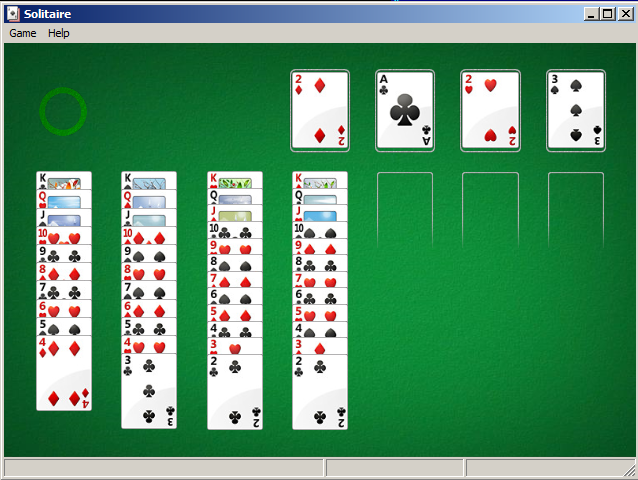
\includegraphics[width=0.6\textwidth]{examples/lines/1.png}
\caption{Обычный вид игры}
\label{fig:lines_1}
\end{figure}

\clearpage
\myindex{\CStandardLibrary!rand()}
Посмотрим, сможем ли мы найти генератор псевдослучайных чисел и и сделать с ним одну шутку.

\IDA быстро распознает стандартную функцию \TT{\_rand} в 
\TT{balltrix.exe} по адресу \TT{0x00403DA0}.
\IDA также показывает, что она вызывается только из одного места:

\lstinputlisting[style=customasmx86]{examples/lines/random.lst}

Назовем её \q{random}.
Пока не будем концентрироваться на самом коде функции.

Эта функция вызывается из трех мест.

Вот первые два:

\lstinputlisting[style=customasmx86]{examples/lines/1.lst}

Вот третье:

\lstinputlisting[style=customasmx86]{examples/lines/2.lst}

Так что у функции только один аргумент.
10 передается в первых двух случаях и 5 в третьем.

Мы также можем заметить, что размер доски 10*10 и здесь 5 возможных цветов.
Это оно!
Стандартная функция \TT{rand()} возвращает число в пределах \TT{0..0x7FFF} и это неудобно, так что многие программисты пишут свою функцию,
возвращающую случайное число в некоторых заданных пределах.
В нашем случае, предел это $0..n-1$ и $n$ передается как
единственный аргумент в функцию.
Мы можем быстро проверить это в отладчике.

Сделаем так, чтобы третий вызов функции всегда возвращал ноль.
В начале заменим три инструкции (\TT{PUSH/CALL/ADD}) 
на \ac{NOP}s.
Затем добавим инструкцию \INS{XOR EAX, EAX}, для очистки регистра \EAX.

\lstinputlisting[style=customasmx86]{examples/lines/fixed.lst}

Что мы сделали, это заменили вызов функции \TT{random()} 
на код, всегда возвращающий ноль.

\clearpage
Теперь запустим:

\begin{figure}[H]
\centering
\includegraphics[width=0.6\textwidth]{examples/lines/2.png}
\caption{Шутка сработала}
\end{figure}

О да, это работает\footnote{Автор этой книги однажды сделал это как 
шутку для его сотрудников, в надежде что они перестанут играть. 
Надежды не оправдались.}.

Но почему аргументы функции \TT{random()} это глобальные переменные?
Это просто потому что в настройках игры можно изменять размер доски, так что эти параметры не фиксированы.
10 и 5 это просто значения по умолчанию.
